%!TEX root = ../thesis.tex

\chapter{Methods}
\label{cha:methods}

\section{Tracking}
\label{sec:methods_tracking}



Point encoding: given the point coordinates $p = (p_x, p_y)$ the generated heatmap $\mathcal{H}$ is as follows:

\begin{equation}
  \mathcal{H}(x, y) = \exp \left[ -4 \log(2) \frac{ (x - p_x)^2 + (y - p_y)^2 }{ \sigma^2 } \right]
\end{equation}


\begin{figure}[h]
\centering
\begin{subfigure}{.5\textwidth}
  \centering
  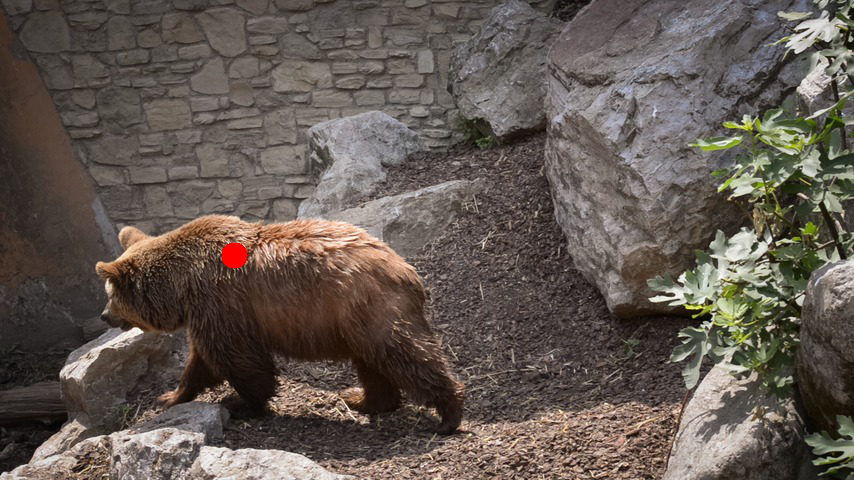
\includegraphics[width=.8\linewidth]{figures/methods/heatmaps/image_point.png}
\end{subfigure}%
\begin{subfigure}{.5\textwidth}
  \centering
  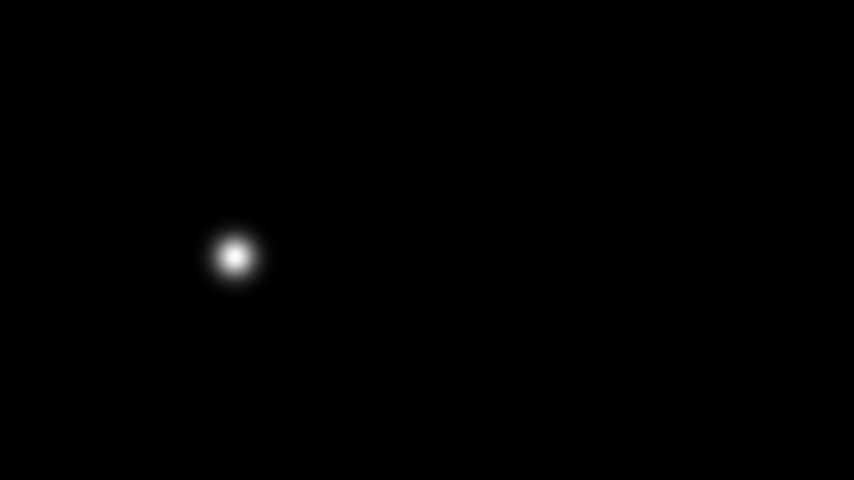
\includegraphics[width=.8\linewidth]{figures/methods/heatmaps/heatmap.png}
\end{subfigure}
\label{fig:point_representation}
\caption{
Point representation.
\textbf{Left}. Image with the annotated points.
\textbf{Right}. Heatmap to represent the point with $\sigma = 32$. }
\end{figure}


\section{Metric Learning with Triplet Loss}
\label{sec:methods_metriclearning}


Metric Learning consists on ...

One way to apply metric learning is using the Triplet Loss. This was first introduced in~\cite{balntas2016learning}.
One famous implementation of this Triplet Loss was used in FaceNet~\cite{schroff2015facenet} where they train a model to embed face images and predict similarity between them.

The triplet loss consists on...anchor positive negative.

\begin{figure}[h]
  \centering
  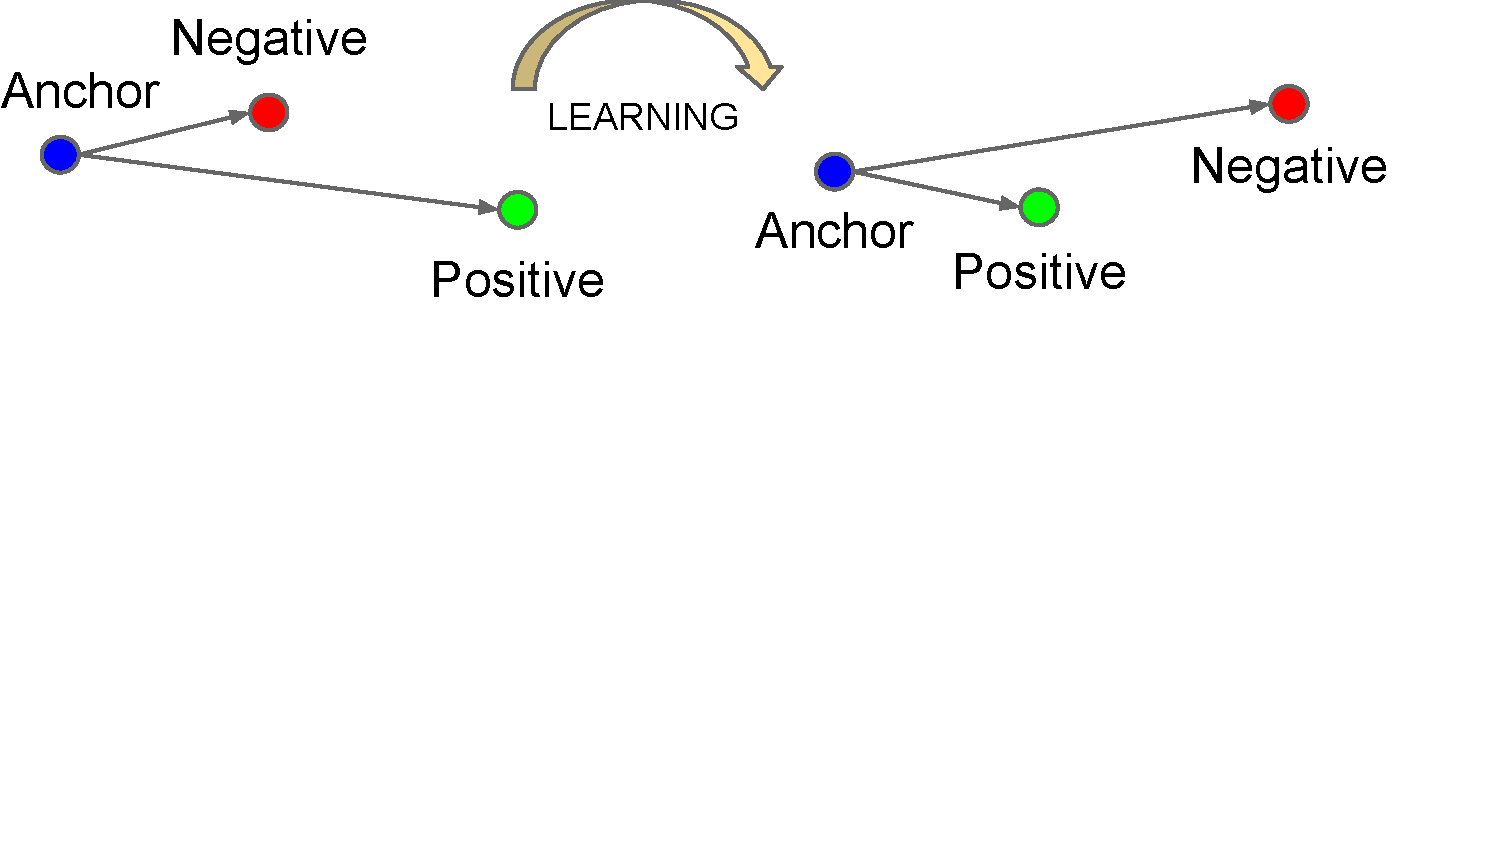
\includegraphics[trim=1cm 10cm 2.5cm 0cm, width=0.7\linewidth]{figures/methods/triplet_loss/triplet_viz.pdf}
  \label{fig:triplet_loss_viz}
  \caption{
    Graphical representation of Triplet Loss learning.
    Figure extracted from~\cite{schroff2015facenet}. }
\end{figure}

In our escenario, we used an embedding model which is a Convolutional Neural Network.
To be more precise, we used the pretrained network from DeepLab~\cite{chen2018deeplab}.
This model has been pretrained with semantic semgnetion from images, and we are using the full network except the last classification part which predicts the pixels class.
Extracting the classifier, we obtain an embedding model that given an image returns an embedding for each pixel at a reduced scale.
The default output size of the model is the same input image size downsampled by 8 and the embeddings present a 2048 dimensionality.
As this dimensionality can be too high, we have tested to plug a convolutional head made of a single convolutional layer with kernel size 1 and its main mission is to reduce the dimensionality to a lower dimension $D$.

Before giving the equations of the Triple Loss, lets define some notation.
Be $\mathcal{I} \in \mathbb{R}^{H \times W}$ the input image of size $H \times W$.
The output size of the model will be $H' \times W' = \frac{H}{8} \times \frac{W}{8}$ and the output embedding will be $\mathcal{X} = \{x_i\}^{H' \times W'}$ where $x_i \in \mathbb{R}^D$ is the i-th output pixel embedding.
Lets be the Convolutional Neural Network as embedding model $f(\mathcal{I}; \Theta)$ which computes the embedding from a single image:

\begin{equation}
  \mathcal{X} = f(\mathcal{I}; \Theta)
\end{equation}

When training the model, there is available the ground truth mask of one object instance in the image. When the image is forwarded throught the model and the embeddings computed, $N$ triplets of pixels are sampled. For each triplet, two pixels with a mask set to 1 are sampled and assigned as anchor and positive pixels ($x_a$ and $x_p$ respectively). Finally a pixel with a mask set to 0 is sampled and assigened as negative pixel $x_n$.

\begin{equation}
  \label{eq:triplet_loss_1}
  \mathcal{L}_{triplet} = \sum_i^N \max \left( d(x_a^{(i)}, x_p^{(i)}) - d(x_a^{(i)}, x_n^{(i)})  + \alpha, 0 \right)
\end{equation}

The $\alpha$ term on the triplet loss is the margin used to inforce the minimum diference between the distance of positive pairs and negative pairs. $d$ is the distance function, which in our case the square of the $l^2$ norm is used. So \eqref{triplet_loss_1} will be as follows:

\begin{equation}
  \label{eq:triplet_loss_2}
  \mathcal{L}_{triplet} =
	\sum_i^N \max \left(
		\|x_a^{(i)} - x_p^{(i)}\|^2_2 - \|x_a^{(i)} - x_n^{(i)}\|_2^2  + \alpha,
		0 \right)
\end{equation}







%%%%%%%%%%%%%%%%%%%%%%%%%%%%%%%%%%%%%%%%%%%%%%%%%%%%%%%%%%%%%%%%%%%%%%555

First study, was to track point on video sequences (DAVIS). Trying different architectures (Hourglass and then ResNet), with different approaches (with and without parent network). First we annotated some points to track, and used and estimation of the heatmap to predict the point (and also multiple scale heatmap).

The second approach was using the ResNet middle representation as representation of the pixel and try to track it.

This led us to pivot and use this representation to segment the instance.
Move the dataset to PASCAL VOC. And introduce the metric learning. Explain the metric learning, its algorithmic sampling. Explain the double triplet sampling.
